% \documentclass[ba,preprint]{imsart}% use this for supplement article
\documentclass[ba]{imsart}
%
\pubyear{2021}
\volume{TBA}
\issue{TBA}
% \doi{0000}
%\arxiv{}
\firstpage{1}
\lastpage{1}

\usepackage{amsthm}
\usepackage{amsmath}
\usepackage{natbib}
\usepackage[colorlinks,citecolor=blue,urlcolor=blue,filecolor=blue,backref=page]{hyperref}
\usepackage{graphicx}


% my added packages: copied from the swiss IJ paper
\usepackage{microtype}
\usepackage{graphicx}
\usepackage{subfigure}
\usepackage{booktabs} % for professional tables
\usepackage{siunitx}
\usepackage{hyperref}
\usepackage{xargs}[2008/03/08]
\usepackage{xfrac}

% adding line numbers.
% delete this when done
\usepackage{lineno}
\linenumbers


% Documentation
% http://ftp.math.purdue.edu/mirrors/ctan.org/macros/latex/contrib/refstyle/refstyle.pdf
\usepackage{refstyle}
\usepackage{varioref} % Use refstyle instead of varioref directly.

% Math scripts
\usepackage{mathrsfs}  % For script fonts
%\usepackage{dutchcal} % Lower-case mathcal
%\usepackage{mathbbol}  % For lower-case bold fonts

% \DeclareFontFamily{OT1}{pzc}{}
% \DeclareFontShape{OT1}{pzc}{m}{it}{<-> s * [1.10] pzcmi7t}{}
% \DeclareMathAlphabet{\mathpzc}{OT1}{pzc}{m}{it}

\usepackage{listings}
\usepackage{pdfpages}

% added packages for todo notes
% pass in option ``disable" to remove notes
\usepackage[textsize=tiny]{todonotes}

% This picks up the knitr boilerplate, allowing us to \input partial knitr
% documents.
\usepackage[]{graphicx}
\usepackage[]{color}
%% maxwidth is the original width if it is less than linewidth
%% otherwise use linewidth (to make sure the graphics do not exceed the margin)
\makeatletter
\def\maxwidth{ %
  \ifdim\Gin@nat@width>\linewidth
    \linewidth
  \else
    \Gin@nat@width
  \fi
}
\makeatother

\definecolor{fgcolor}{rgb}{0.345, 0.345, 0.345}
\newcommand{\hlnum}[1]{\textcolor[rgb]{0.686,0.059,0.569}{#1}}%
\newcommand{\hlstr}[1]{\textcolor[rgb]{0.192,0.494,0.8}{#1}}%
\newcommand{\hlcom}[1]{\textcolor[rgb]{0.678,0.584,0.686}{\textit{#1}}}%
\newcommand{\hlopt}[1]{\textcolor[rgb]{0,0,0}{#1}}%
\newcommand{\hlstd}[1]{\textcolor[rgb]{0.345,0.345,0.345}{#1}}%
\newcommand{\hlkwa}[1]{\textcolor[rgb]{0.161,0.373,0.58}{\textbf{#1}}}%
\newcommand{\hlkwb}[1]{\textcolor[rgb]{0.69,0.353,0.396}{#1}}%
\newcommand{\hlkwc}[1]{\textcolor[rgb]{0.333,0.667,0.333}{#1}}%
\newcommand{\hlkwd}[1]{\textcolor[rgb]{0.737,0.353,0.396}{\textbf{#1}}}%
\let\hlipl\hlkwb

\usepackage{framed}
\makeatletter
\newenvironment{kframe}{%
 \def\at@end@of@kframe{}%
 \ifinner\ifhmode%
  \def\at@end@of@kframe{\end{minipage}}%
  \begin{minipage}{\columnwidth}%
 \fi\fi%
 \def\FrameCommand##1{\hskip\@totalleftmargin \hskip-\fboxsep
 \colorbox{shadecolor}{##1}\hskip-\fboxsep
     % There is no \\@totalrightmargin, so:
     \hskip-\linewidth \hskip-\@totalleftmargin \hskip\columnwidth}%
 \MakeFramed {\advance\hsize-\width
   \@totalleftmargin\z@ \linewidth\hsize
   \@setminipage}}%
 {\par\unskip\endMakeFramed%
 \at@end@of@kframe}
\makeatother

\definecolor{shadecolor}{rgb}{.97, .97, .97}
\definecolor{messagecolor}{rgb}{0, 0, 0}
\definecolor{warningcolor}{rgb}{1, 0, 1}
\definecolor{errorcolor}{rgb}{1, 0, 0}
\newenvironment{knitrout}{}{} % an empty environment to be redefined in TeX

\usepackage{alltt}


\startlocaldefs
% This defines math macros.

% Operators
\def\mbe{\mathbb{E}}%
\def\ind#1{\mathbb{I}\left(#1\right)}
\def\evalat#1#2{\left.#1\right|_{#2}}
\def\fracat#1#2#3{\left.\frac{#1}{#2}\right\vert_{#3}}
\def\iid{\overset{iid}{\sim}}
\def\expect#1#2{\underset{#1}{\mathbb{E}}\left[#2\right]}
\def\cov#1#2{\underset{#1}{\mathrm{Cov}}\left(#2\right)}
\def\expecthat#1#2{\underset{#1}{\widehat{\mathbb{E}}}\left[#2\right]}
\def\abs#1{\left|#1\right|}
\def\norm#1{\left\Vert#1\right\Vert}
\def\norminf#1{\left\Vert#1\right\Vert_{\infty}}
\def\sumk{\sum_{\k=1}^{\kmax}}
\def\sumkm{\sum_{\k=1}^{\kmax - 1}}
\def\dirderiv#1#2{\delta_{#1\rightarrow#2}} % A directional derivative (unused?)
\def\linop{\mathcal{L}} % A linear operator

\DeclareMathOperator*{\argmax}{\mathrm{argmax}}
\DeclareMathOperator*{\argmin}{\mathrm{argmin}}
\DeclareMathOperator*{\esssup}{\mathrm{esssup}}

% Variables
\def\etaopt{\hat\eta} % Optimal vb parameters
\def\x{x}   % Data
\def\t{t}   % Generic priur parameter
\def\z{z}   % Cluster indicators
\def\g{g}   % Function of interest
\def\k{k}   % Cluster index
\def\n{n}   % Data index
\def\nuk{\nu_{\k}}   % K-th stick.  Have to type this a lot.
\def\const{C}   % Constant
\def\lnu{\tilde{\nu}}   % Unconstrained stick
\def\lnumean{\eta^{\mu}}   % Unconstrained stick vb mean
\def\lnusd{\eta^{\sigma}}   % Unconstrained stick vb std
\def\hess#1{H_{#1}}   % Hessian
\def\phiz{0_\phi}   % The phi zero function.
\def\infl{\psi}   % The influence function
\def\inflg{\psi_{\g}}   % The influence function for a function of interest

\def\etatheta{\eta_{\theta}}  % VB parameters for certain components
\def\etanu{\eta_{\nu}}  % VB parameters for certain components
\def\etanuk{\eta_{\nuk}}  % VB parameters for certain components
\def\etaz{\eta_{\z}}  % VB parameters for certain components
\def\etaglob{\eta_{\gamma}}  % VB parameters for theta and nu
\def\etaopttheta{\etaopt_{\theta}}  % VB parameters for certain components
\def\etaoptnu{\etaopt_{\nu}}  % VB parameters for certain components
\def\etaoptnuk{\etaopt_{\nuk}}  % VB parameters for certain components
\def\etaoptz{\etaopt_{\z}}  % VB parameters for certain components
\def\etaoptgamma{\etaopt_{\gamma}}  % VB parameters for certain components


% Distributions
\def\pstick{p_{\mathrm{stick}}}   % Stick breaking distribution
\def\q{q}   % VB dist
\def\logp{\ell}   % Log probabiltty
\def\lqgrad#1{{\nabla \log \q}\left(#1\right)}   % Log VB distribution gradient
\def\lqhess#1{{\nabla^2 \log \q}\left(#1\right)}   % Log VB distribution Hessian
\def\lqgradbar#1{\overline{\lqgrad{#1}}\,\,}   % Log VB distribution gradient centered
\def\lqhessbar#1{\overline{\lqhess{#1}}\,\,}   % Log VB distribution Hessian centered
\def\normdist#1{\mathcal{N}\left(#1\right)}   % Normal distribution
\def\KL#1{\mathrm{KL}\left(#1\right)}   % KL divergence
\def\KLgrad#1{\mathrm{KL}_{\eta}\left(#1\right)}   % KL divergence
\def\KLhess#1{\mathrm{KL}_{\eta\eta}\left(#1\right)}   % KL divergence
\def\wishart#1{\mathrm{Wishart}\left(#1\right)}   % Wishart distribution
\def\gammadist#1{\mathrm{Gamma}\left(#1\right)}   % Gamma distribution
\def\betadist#1{\mathrm{Beta}\left(#1\right)}   % Gamma distribution
\def\pb{p_{0}}   % Base prior
\def\pa{p_{1}}   % Alternative prior

% Taylor series
\def\etalin{\etaopt^{\mathrm{lin}}}
\def\glin{\g^{\mathrm{lin}}}
\def\gapprox{\g^{\etalin}}

% Dimensions
\def\N{N}   % Number of datapoints
\def\K{K}   % Number of components
\def\kmax{{\K_{\mathrm{max}}}}   % Truncation
\def\etadim{{D_{\eta}}}
\def\thetadim{{D_{\theta}}}
\def\zetadim{{D_{\zeta}}}
\def\ngh{N_{\mathrm{GH}}}   % Number of GH points

% Domains
\def\etadom{\Omega_{\eta}}
\def\thetadom{\Omega_{\theta}}
\def\tdom{\Omega_{\t}}
\def\linf{{L_{\infty}[0,1]}}
\def\ball{\mathcal{B}}

% Annotations
\def\mathtxt#1{\quad\textrm{#1}\quad}%
\def\mathand{\quad\textrm{and}\quad}%
\def\mathwhere{\quad\textrm{where}\quad}%
\def\constdesc#1{\textrm{(}\const\textrm{ does not depend on }#1\textrm{)}}
\def\assuitemref#1#2{\assuref{#1} (\itemref{#2})}%


% This specifies the formatting for references (sections, theorems, etc.)

%%%%%%%%%%%%%%%%%%%%
% amsthm commands

\theoremstyle{plain}
\newtheorem{lem}{Lemma}
\newtheorem{thm}{Theorem}
\newtheorem{prop}{Proposition}
\newtheorem{cond}{Condition}
\newtheorem{assu}{Assumption}
\newtheorem{cor}{Corollary}
\newtheorem{conj}{Conjecture}

%\theoremstyle{definition}
% \newtheorem{defn}{Definition}
%\newtheorem{ex}{Example}

% Example environment with a terminating symbol.
% https://tex.stackexchange.com/questions/16453/denoting-the-end-of-example-remark
\theoremstyle{definition}
\newtheorem{examplex}{Example}
\newenvironment{ex}
  {\pushQED{\qed}\renewcommand{\qedsymbol}{$\triangle$}\examplex}
  {\popQED\endexamplex}

\theoremstyle{definition}
\newtheorem{defnx}{Definition}
\newenvironment{defn}
    {\pushQED{\qed}\renewcommand{\qedsymbol}{$\boxdot$}\defnx}
    {\popQED\enddefnx}


\newcommand{\seeproof}[1]{(See \proofref{#1} \proofpageref[vref]{#1}.)}
\newcommand{\proofof}[1]{\noindent{\bf Proof of #1.}}


%%%%%%%%%%%%%%%%%%%%
% refstyle commands

\newref{event}{
    name=Event~, %
    names=Events~, %
    Name=Event~,
    Names=Events~
    }

\newref{item}{
    name=Item~, %
    names=Items~, %
    Name=Item~,
    Names=Items~
    }

\newref{fig}{
    name=Figure~, %
    Name=Figure~
    }

\newref{tab}{
    name=Table~, %
    Name=Table~
    }

\newref{sec}{
    name=Section~, %
    Name=Section~,
    names=Sections~,
    Names=Sections~,
    }

\newref{app}{
    name=Appendix~, %
    Name=Appendix~
    }

\newref{eq}{
    name=Eq.~, %
    Name=Eq.~,
    names=Eqs.~, %
    Names=Eqs.~
    }

\newref{fig}{
    name=Figure~, %
    Name=Figure~,
    names=Figures~, %
    Names=Figures~,
    }

\newref{def}{
    name=Definition~, %
    Name=Definition~
    }

\newref{assu}{
    name=Assumption~, %
    Name=Assumption~,
    names=Assumptions~, %
    Names=Assumptions~,
    }

\newref{cond}{
    name=Condition~, %
    Name=Condition~,
    names=Conditions~, %
    Names=Conditions~
    }

\newref{prop}{
    name=Proposition~, %
    Name=Proposition~,
    names=Propositions~, %
    Names=Propositions~
    }

\newref{lem}{
    name=Lemma~, %
    Name=Lemma~,
    names=Lemmas~, %
    Names=Lemmas~
    }

\newref{ex}{
    name=Example~, %
    Name=Example~,
    names=Examples~,
    Names=Examples
    }

\newref{cory}{
    name=Corollary~, %
    Name=Corollary~
    }

\newref{thm}{
    name=Theorem~, %
    Name=Theorem~,
    names=Theorems~, %
    Names=Theorems~
    }

\newref{proof}{
    name=Proof~, %
    Name=Proof~
    }

\newref{conj}{
    name=Conjecture~, %
    Name=Conjecture~
    }

\newref{algr}{
    name=Algorithm~, %
    Name=Algorithm~,
    names=Algorithms~, %
    Names=Algorithms~,
    }


%% refstyle examples:
% \Secref[vref]{introduction} contains \secref{introduction}.
% \Secref[vref]{ack} does not contain \secref{introduction}.
%
% \begin{align}
%     x=y \eqlabel{myeq}
% \end{align}
%

\endlocaldefs

\begin{document}

% Output of the knitr file defining certain simulated figures.
%%%%%%%%%%%%%%%%%%%%%%%%%%%%%%%%%%%%%%
%%%%%%%%%%%%%%%%%%%%%%%%%%%%%%%%%%%%%%
% Do not edit the TeX file your work
% will be overwritten.  Edit the RnW
% file instead.
%%%%%%%%%%%%%%%%%%%%%%%%%%%%%%%%%%%%%%
%%%%%%%%%%%%%%%%%%%%%%%%%%%%%%%%%%%%%%



\newcommand{\SimPathologicalRTwoFig}{

\begin{knitrout}
\definecolor{shadecolor}{rgb}{0.969, 0.969, 0.969}\color{fgcolor}\begin{figure}[!h]

{\centering 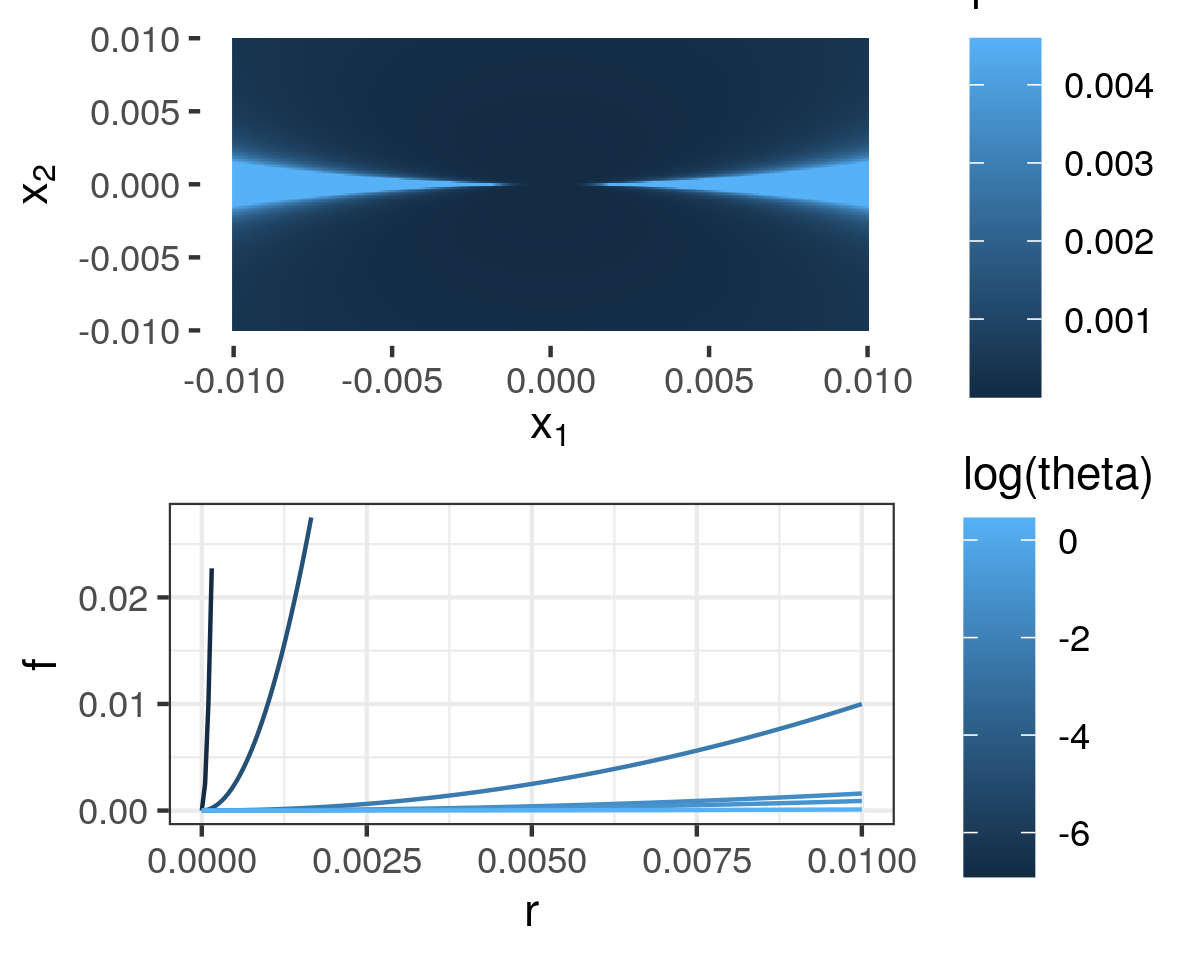
\includegraphics[width=0.980\linewidth,height=0.784\linewidth]{figure/r2_pathological-1} 

}

\caption[A plot of $f(x_1, x_2)$ from \exref{r2_pathological}]{A plot of $f(x_1, x_2)$ from \exref{r2_pathological}.}\label{fig:r2_pathological}
\end{figure}


\end{knitrout}
}


\newcommand{\SimPositivePertFig}{

\begin{knitrout}
\definecolor{shadecolor}{rgb}{0.969, 0.969, 0.969}\color{fgcolor}\begin{figure}[!h]

{\centering 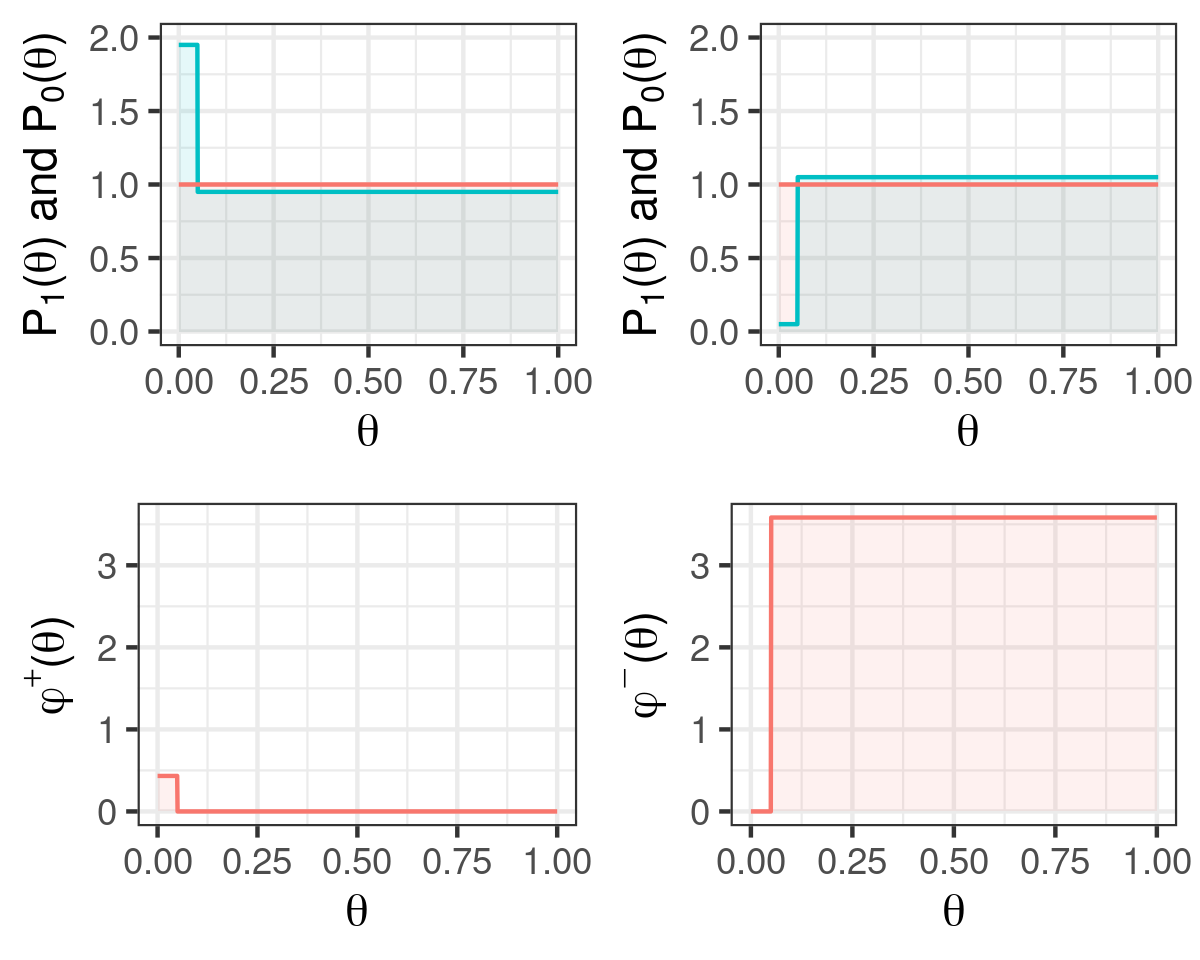
\includegraphics[width=0.980\linewidth,height=0.784\linewidth]{figure/positive_pert-1} 

}

\caption{A plot of the perturbations from \exref{positive_pert_large} with $p=2$ and $\epsilon=0.05$.  Positive $\phi$ can only add mass, so to remove a small amount of mass requires adding mass everywhere else and re-normalizing, resulting in a large perturbation according to $\norm{\cdot}_p$.}\label{fig:positive_pert}
\end{figure}


\end{knitrout}
}


\newcommand{\FunctionPathsFig}{

\begin{knitrout}
\definecolor{shadecolor}{rgb}{0.969, 0.969, 0.969}\color{fgcolor}\begin{figure}[!h]

{\centering 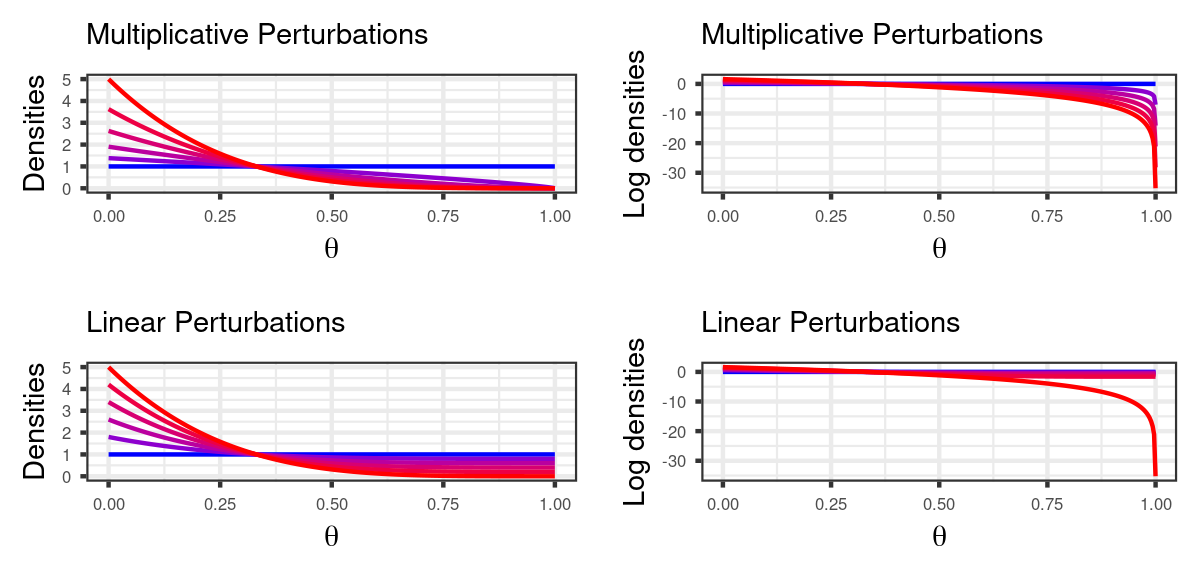
\includegraphics[width=0.980\linewidth,height=0.470\linewidth]{figure/path-1} 

}

\caption[Multiplicative and linear mixture paths between two densities]{Multiplicative and linear mixture paths between two densities.}\label{fig:path}
\end{figure}


\end{knitrout}
}


\newcommand{\FunctionPathsMultFig}{

\begin{knitrout}
\definecolor{shadecolor}{rgb}{0.969, 0.969, 0.969}\color{fgcolor}\begin{figure}[!h]

{\centering 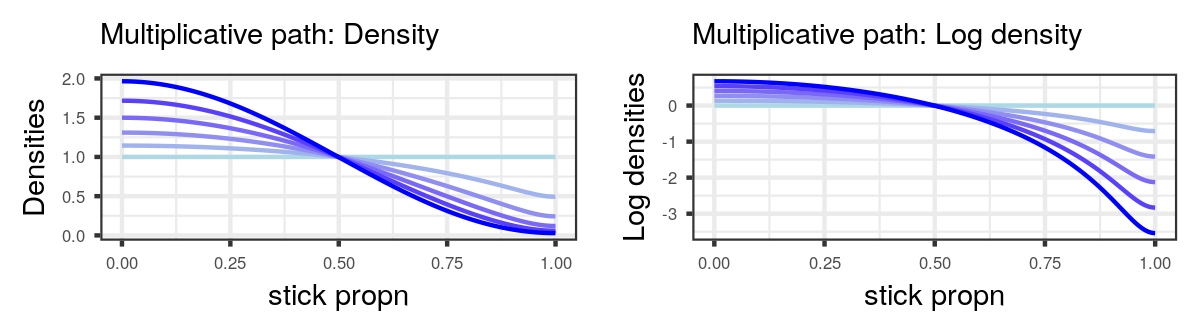
\includegraphics[width=0.980\linewidth,height=0.274\linewidth]{figure/mult_path-1} 

}

\caption[Multiplicative mixture paths between two densities]{Multiplicative mixture paths between two densities.}\label{fig:mult_path}
\end{figure}


\end{knitrout}
}


\newcommand{\FunctionPathsLinFig}{

\begin{knitrout}
\definecolor{shadecolor}{rgb}{0.969, 0.969, 0.969}\color{fgcolor}\begin{figure}[!h]

{\centering 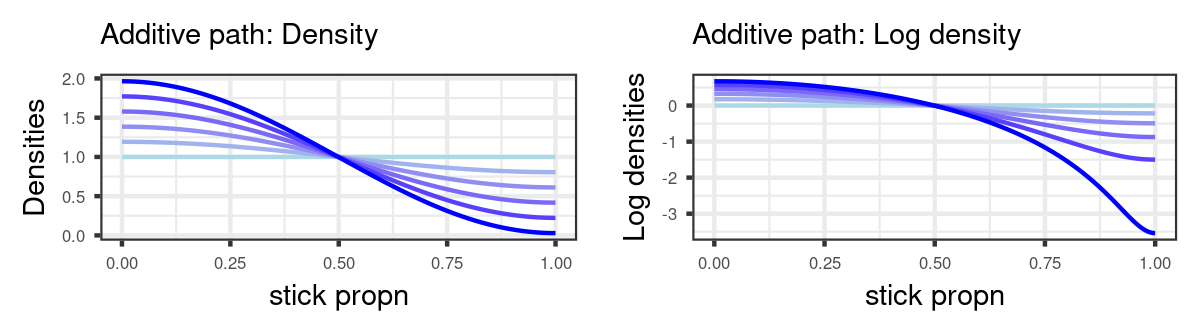
\includegraphics[width=0.980\linewidth,height=0.274\linewidth]{figure/lin_path-1} 

}

\caption[Linear mixture paths between two densities]{Linear mixture paths between two densities.}\label{fig:lin_path}
\end{figure}


\end{knitrout}
}


\newcommand{\FunctionBallFig}{

\begin{knitrout}
\definecolor{shadecolor}{rgb}{0.969, 0.969, 0.969}\color{fgcolor}\begin{figure}[!h]

{\centering 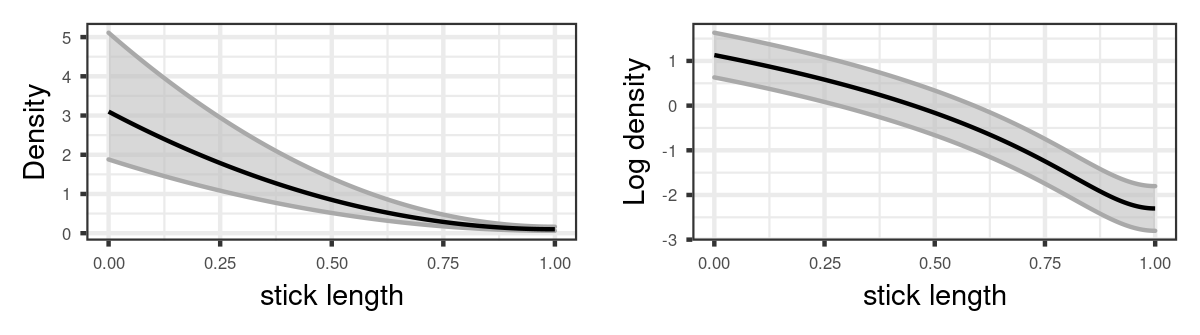
\includegraphics[width=0.980\linewidth,height=0.274\linewidth]{figure/func_ball-1} 

}

\caption[An $\linf{\cdot}$ ball]{An $\linf{\cdot}$ ball.}\label{fig:func_ball}
\end{figure}


\end{knitrout}
}


%% *** Frontmatter ***

\begin{frontmatter}
\title{Evaluating Sensitivity to the Stick Breaking Prior in Bayesian Nonparametrics}
%\title{\support{}}
\runtitle{BNP sensitivity}

\begin{aug}
\author{\fnms{Ryan} \snm{Giordano}\thanksref{addr1,t1}},
\author{\fnms{Runjing} \snm{Liu}\thanksref{addr2,t1}},
\author{\fnms{Michael I.} \snm{Jordan}\thanksref{addr2}},
\and
\author{\fnms{Tamara} \snm{Broderick}\thanksref{addr1}}
%\author{\fnms{<firstname>} \snm{<surname>}\thanksref{}\ead[label=e1]{}}
%\and
%\author{\fnms{} \snm{}}

\runauthor{}

\address[addr1]{Department of EECS, MIT
77 Massachusetts Ave., 38-401
Cambridge, MA 02139}

\address[addr2]{Department of Statistics, UC Berkeley
367 Evans Hall, UC Berkeley
Berkeley, CA 94720}

\thankstext{t1}{Equal contribution. }

\end{aug}

\begin{abstract}

The Dirichlet process has become a mainstay in unsupervised learning tasks
like clustering and topic modeling. Its stick-breaking representation in particular lends itself
to fast approximate posterior inference with variational Bayes. However, choices for the
stick-breaking representation are often made from convenience. For instance, particular
values of the concentration parameter are favored by different applications, and the beta
distribution of the sticks lends itself to conditional conjugacy and closed-form inferential updates.
In many cases, though, different values of the concentration parameter and the underlying stick-breaking
distribution could equally align with prior beliefs. If the major conclusions of our analysis changed under these different reasonable choices, we might worry that our conclusions were driven by arbitrary implementation choices rather than meaningful data trends.
In the present work we demonstrate how to assess the sensitivity of conclusions
to the choice of concentration parameter and stick-breaking distribution. While we focus on perturbations to stick-breaking priors in Bayesian nonparametrics, along the way we develop new theory to support sensitivity analysis more generally for variational Bayes.
\end{abstract}

%% ** Keywords **
\begin{keyword}%[class=MSC]
%\kwd{}
%\kwd[]{}
\end{keyword}

\end{frontmatter}

%% ** Mainmatter **

%\section{}\label{}

% \begin{figure}
% \includegraphics{<eps-file>}% place <eps-file> in ./img  subfolder
% \caption{}
% \label{}
% \end{figure}


% \begin{table}
% *****************
% \begin{tabular}{lll}
% \end{tabular}
% *****************
% \caption{}
% \label{}
% \end{figure}

%%%%%%%%%%%%%%%%%%%%%%%%%%%%%%%%%%%%%%%%%%%%%%
%% Supplementary Material, if any, should   %%
%% be provided in {supplement} environment  %%
%% with title and short description.        %%
%%%%%%%%%%%%%%%%%%%%%%%%%%%%%%%%%%%%%%%%%%%%%%
%\begin{supplement}
%\stitle{???}
%\sdescription{???.}
%\end{supplement}

%% ** The bibliograhy **
%\bibliographystyle{ba}
%\bibliography{<bib-data-file>}% place <bib-data-file> in ./bib folder

% ** Acknowledgements **
%\begin{acks}[Acknowledgments]
%\end{acks}


\end{document}
